\chapter{Algebra}

\section{Group Theory}
% hi
\begin{example}
    Give an example of an element that has a right inverse but not a left inverse.
    \begin{equation*}
        \begin{bmatrix}
            1&0
        \end{bmatrix}\begin{bmatrix}
            1\\
            0
        \end{bmatrix}=\begin{bmatrix}
            1
        \end{bmatrix}
    \end{equation*}
\end{example}
We note that the permutations (bijective maps from $T$ to $T$) of a set $T$ form a group, under composition of maps. Now we remind the definition of symmetric groups.
\begin{defn}[Symmetric group]
    Let the group of permutations of the set of indices $\{1,2, \ldots, n\}$ is called the symmetric group, denoted by $S_n$. And if $n$ is finite, then $|S_n|=n!$.
\end{defn}
There is only one group of order 2, because every group can be shown to have the form $\{1, g\}$, which is $S_2$. For $S_3$, it is the smallest group that the law of composition isn't commutative.

\begin{prop}
    Any subgroup of the additive integers is of the form 
    \begin{equation*}
        \{a\mathbb{Z}: a\in\mathbb{Z}\}
    \end{equation*}
\end{prop}
\begin{prop}
    For $a,b\in\mathbb{Z}$ such that $d$ is the greatest common divisor of $a,b$, i.e., $d=gcd(a,b)$, then 
\begin{equation*}
    \Z d=\Z a+\Z b
\end{equation*}
\end{prop}
This is because for $d=gcd(a,b)$, there exists integers $s,t$ such that $d=sa+tb$. This implies that if $a,b$ are coprime, then the subgroup of $\Z$ that contains both $a,b$ is $\Z$ itself.

\begin{example}
    $\begin{bmatrix}
        1&1\\
        0&1
    \end{bmatrix}$
    has infinite order in GL$_2$.
\end{example}
\begin{example}
    The simplest group that is not cyclic. The Klein four group consisting of 4 elements:
    \begin{equation*}
        \begin{bmatrix}
            \pm 1&0\\
            0 &\pm 1
        \end{bmatrix}
    \end{equation*}
\end{example}
\begin{prob}
    Suppose $a,b\in G$, then $ab$ and $ba$ have the same order.
\end{prob}
This can be done by expanding out the terms.

\begin{prob}
    A cyclic group of order $n$ contains $\phi(n)$ of generators, where $\phi(n)$ is the positive integers that are relatively prime to $n$, less than $n$.
\end{prob}

\begin{prob}
    The product of two elements of finite order could be an element of infinite order. 
\end{prob}
\begin{proof}
    \begin{equation*}
        \begin{bmatrix}
            0&1\\
            1&0
        \end{bmatrix},
        \begin{bmatrix}
            0&2\\
            \frac{1}{2}&0
        \end{bmatrix}
    \end{equation*}
    Their product is $\begin{bmatrix}
        \frac{1}{2}&0\\
        0&2
    \end{bmatrix}$.
\end{proof}

\begin{defn}[subgroup]
    $H$ is a subgroup of $G$ if and only if for any $a,b\in H$, $ab^{-1}\in H$.
\end{defn}
\begin{prop}
    If $1$ is the identity of a subgroup $H$ of $G$, then $1$ is the identity of $G$ as well.
\end{prop}
This can be used to show that if $\phi: G\to G'$ is a homomorphism, then $\phi(1_G)=1_{G'}$. One can show that $1_{G'}$ is the identity of the subgroup $Im(\phi)$.

\begin{defn}
    The kernel of a homomorphism $\phi$ is 
    \begin{equation*}
        \{g\in G: \phi(g)=1\}
    \end{equation*}
\end{defn}
\begin{defn}
    The alternating group $A_n$ is the group of even permutations, i.e., having an even number of two-element swaps. Alternatively, it is the kernel of the sign homomorphism $S_n\to \{-1, 1\}$ (it only has positive 1 determinant).
\end{defn}

\begin{defn}
    A subgroup $N$ is normal if for every $a\in N$, and every $g\in G$, $gag^{-1}\in N$.
\end{defn}

\begin{prop}
    The kernel of the map from $G\to Aut(G)$
    \begin{equation*}
        g\mapsto f_g(h)=ghg^{-1}
    \end{equation*}
    The kernel of this map is all the elements $g$ such that $gh=hg$, which is called the center $Z$ of $G$. It is a normal subgroup.
\end{prop}


\begin{prop}
    The conjugate map $\varphi:G\to G$ is an automorphism, i.e., it is an isomorphism onto itself. 
    \begin{equation*}
        \varphi(x)=gxg^{-1}
    \end{equation*}
    for some $g\in G$.
\end{prop}
\begin{proof}
    The inverse map is given by conjuation by $g^{-1}$, hence is bijective. Homomorphism is easy to check.
\end{proof}
We note that two elements $a,b$ commute if and only if $aba^{-1}=b$.



\begin{defn}[fibers]
    Let $f:S\to T$ be bijective, then define the preimage of a particular element as the fibers of $f$.
    \begin{equation*}
        f^{-1}(t)=\{s\in S: f(s)=t\}
    \end{equation*}
\end{defn}
\begin{center}
    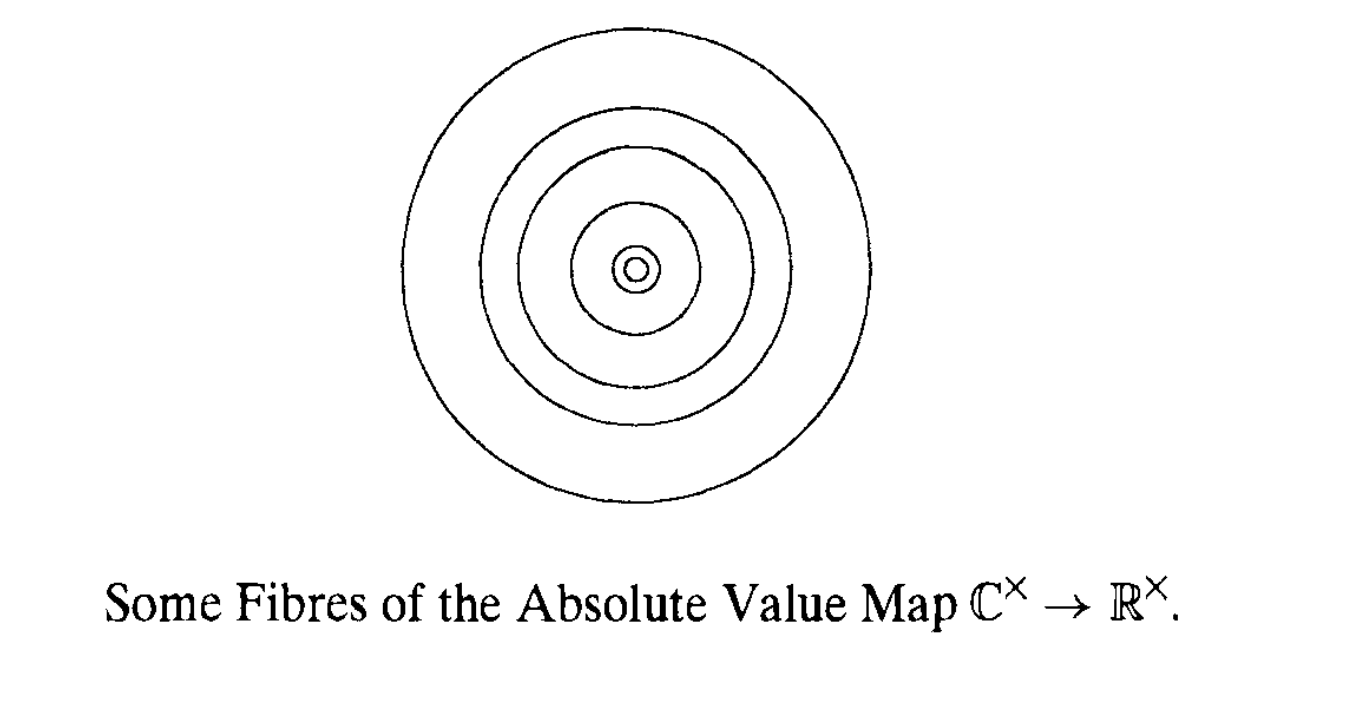
\includegraphics[width=6cm, height=3cm]{fiber.png}
\end{center}
The fibers define an equivalence relation. In other words, two elements $a, b$ are equivalent, $a\sim b$ if and only if $f(a)=f(b)$.

Let $\varphi:G\to G'$ be a homomorphism, then the fibers are given by the cosets $aK$, where $K$ is the kernel of $\varphi$.

\begin{prop}
    The order of an element $a\in G$ divides the order of the group $G$.
\end{prop}
\begin{proof}
    The order of an element $a$ is the same as the number of elements of $\langle a\rangle$, which is the cyclic group generated by $a$. By Lagrange's theorem, the order of the subgroup divides the order of the group.
\end{proof}

\begin{prop}
    Let $\varphi:G\to G'$ be a homomorphism for a finite group, then 
    \begin{equation*}
        |G|=|ker(\varphi)|\cdot |Im(\varphi)|
    \end{equation*}
\end{prop}
\begin{proof}
    This follows by cosets partition $G$ and Lagrange's theorem.
\end{proof}




